% !TeX spellcheck = es_MX
\documentclass[12pt, a4paper, titlepage]{report}
\usepackage[spanish]{babel}
\usepackage[utf8]{inputenc}
\usepackage[linesnumbered,lined,boxed,commentsnumbered]{algorithm2e}
\usepackage{enumitem,kantlipsum}
\usepackage{array}
\usepackage{placeins}
% Códigos y codificación para caracteres en español
\usepackage{listings}
\usepackage{color}
\lstset{literate=
	{á}{{\'a}}1 {é}{{\'e}}1 {í}{{\'i}}1 {ó}{{\'o}}1 {ú}{{\'u}}1
	{Á}{{\'A}}1 {É}{{\'E}}1 {Í}{{\'I}}1 {Ó}{{\'O}}1 {Ú}{{\'U}}1
	{à}{{\`a}}1 {è}{{\`e}}1 {ì}{{\`i}}1 {ò}{{\`o}}1 {ù}{{\`u}}1
	{À}{{\`A}}1 {È}{{\'E}}1 {Ì}{{\`I}}1 {Ò}{{\`O}}1 {Ù}{{\`U}}1
	{ä}{{\"a}}1 {ë}{{\"e}}1 {ï}{{\"i}}1 {ö}{{\"o}}1 {ü}{{\"u}}1
	{Ä}{{\"A}}1 {Ë}{{\"E}}1 {Ï}{{\"I}}1 {Ö}{{\"O}}1 {Ü}{{\"U}}1
	{â}{{\^a}}1 {ê}{{\^e}}1 {î}{{\^i}}1 {ô}{{\^o}}1 {û}{{\^u}}1
	{Â}{{\^A}}1 {Ê}{{\^E}}1 {Î}{{\^I}}1 {Ô}{{\^O}}1 {Û}{{\^U}}1
	{œ}{{\oe}}1 {Œ}{{\OE}}1 {æ}{{\ae}}1 {Æ}{{\AE}}1 {ß}{{\ss}}1
	{ű}{{\H{u}}}1 {Ű}{{\H{U}}}1 {ő}{{\H{o}}}1 {Ő}{{\H{O}}}1
	{ç}{{\c c}}1 {Ç}{{\c C}}1 {ø}{{\o}}1 {å}{{\r a}}1 {Å}{{\r A}}1
	{€}{{\EUR}}1 {£}{{\pounds}}1
}
%%Appendix
\usepackage[toc,page]{appendix}

%%Tablas
\usepackage{tabularx}

%%otros
\usepackage{float}
\usepackage{subfig}
\usepackage{comment}

% http://ctan.org/pkg/booktabs
\usepackage{booktabs}
\newcommand{\tabitem}{~~\llap{\textbullet}~~}

%%Imágenes
\usepackage{graphicx}

%%Colores de texto 
\usepackage{xcolor}
\usepackage{colortbl}

%%Links
\usepackage[hidelinks]{hyperref}

%%Comentarios
\usepackage{verbatim}

%%PARA IMÁGENES EN LÍNEA
%\usepackage[english]{babel}

%%Acrónimos
\usepackage[acronym]{glossaries}

%%Glosario
\usepackage{glossaries}

\usepackage{pdfpages}

%%ESTILO DE CÓDIGO
\lstdefinestyle{codeStyle}{
	backgroundcolor=\color{backcolour}, commentstyle=\color{commentcolor},
	keywordstyle=\color{guindapoli},
	numberstyle=\tiny\color{azulescom},
	stringstyle=\color{azulfuerte},
	basicstyle=\ttfamily\footnotesize,
	breakatwhitespace=false, 
	breaklines=true, 
	captionpos=b,
	keepspaces=true,
	numbers=left,
	numbersep=5pt,
	showspaces=false,
	showstringspaces=false,
	showtabs=false,
	tabsize=3
}
\definecolor{delim}{RGB}{20,105,176}

%% JSON
\lstdefinelanguage{json}{
	basicstyle=\normalfont\ttfamily,
	numbers=left,
	numberstyle=\tiny\color{azulescom},
	stringstyle=\color{azulfuerte},
	stepnumber=1,
	numbersep=8pt,
	showstringspaces=false,
	breaklines=true,
	backgroundcolor=\color{backcolour},
	literate=
	*{0}{{{\color{azulfuerte}0}}}{1}
	{1}{{{\color{azulfuerte}1}}}{1}
	{2}{{{\color{azulfuerte}2}}}{1}
	{3}{{{\color{azulfuerte}3}}}{1}
	{4}{{{\color{azulfuerte}4}}}{1}
	{5}{{{\color{azulfuerte}5}}}{1}
	{6}{{{\color{azulfuerte}6}}}{1}
	{7}{{{\color{azulfuerte}7}}}{1}
	{8}{{{\color{azulfuerte}8}}}{1}
	{9}{{{\color{azulfuerte}9}}}{1}
	{:}{{{\color{guindapoli}{:}}}}{1}
	{,}{{{\color{guindapoli}{,}}}}{1}
	{\{}{{{\color{guindapoli}{\{}}}}{1}
	{\}}{{{\color{guindapoli}{\}}}}}{1}
	{[}{{{\color{guindapoli}{[}}}}{1}
	{]}{{{\color{guindapoli}{]}}}}{1},
}

\lstset{style=codeStyle}


\definecolor{lightgray}{rgb}{.9,.9,.9}
\definecolor{darkgray}{rgb}{.4,.4,.4}
\definecolor{purple}{rgb}{0.65, 0.12, 0.82}

%% Javascript
\lstdefinelanguage{JavaScript}{
	keywords={typeof, new, true, false, catch, function, return, null, catch, switch, var, if, in, while, do, else, case, break, let, continue},
	keywordstyle=\color{blue}\bfseries,
	ndkeywords={class, export, boolean, throw, implements, import, this},
	ndkeywordstyle=\color{darkgray}\bfseries,
	identifierstyle=\color{black},
	sensitive=false,
	comment=[l]{//},
	morecomment=[s]{/*}{*/},
	commentstyle=\color{purple}\ttfamily,
	stringstyle=\color{red}\ttfamily,
	morestring=[b]',
	morestring=[b]"
}

\lstset{
	language=JavaScript,
	backgroundcolor=\color{lightgray},
	extendedchars=true,
	basicstyle=\footnotesize\ttfamily,
	showstringspaces=false,
	showspaces=false,
	numbers=left,
	numberstyle=\footnotesize,
	numbersep=9pt,
	tabsize=2,
	breaklines=true,
	showtabs=false,
	captionpos=b
}
%% ESTO ES PYTHON

\definecolor{maroon}{cmyk}{0, 0.87, 0.68, 0.32}
\definecolor{halfgray}{gray}{0.55}
\definecolor{ipython_frame}{RGB}{207, 207, 207}
\definecolor{ipython_bg}{RGB}{247, 247, 247}
\definecolor{ipython_red}{RGB}{186, 33, 33}
\definecolor{ipython_green}{RGB}{0, 128, 0}
\definecolor{ipython_cyan}{RGB}{64, 128, 128}
\definecolor{ipython_purple}{RGB}{170, 34, 255}

\lstset{
	breaklines=true,
	extendedchars=true,
	literate=
	{á}{{\'a}}1 {é}{{\'e}}1 {í}{{\'i}}1 {ó}{{\'o}}1 {ú}{{\'u}}1
	{Á}{{\'A}}1 {É}{{\'E}}1 {Í}{{\'I}}1 {Ó}{{\'O}}1 {Ú}{{\'U}}1
	{à}{{\`a}}1 {è}{{\`e}}1 {ì}{{\`i}}1 {ò}{{\`o}}1 {ù}{{\`u}}1
	{À}{{\`A}}1 {È}{{\'E}}1 {Ì}{{\`I}}1 {Ò}{{\`O}}1 {Ù}{{\`U}}1
	{ä}{{\"a}}1 {ë}{{\"e}}1 {ï}{{\"i}}1 {ö}{{\"o}}1 {ü}{{\"u}}1
	{Ä}{{\"A}}1 {Ë}{{\"E}}1 {Ï}{{\"I}}1 {Ö}{{\"O}}1 {Ü}{{\"U}}1
	{â}{{\^a}}1 {ê}{{\^e}}1 {î}{{\^i}}1 {ô}{{\^o}}1 {û}{{\^u}}1
	{Â}{{\^A}}1 {Ê}{{\^E}}1 {Î}{{\^I}}1 {Ô}{{\^O}}1 {Û}{{\^U}}1
	{œ}{{\oe}}1 {Œ}{{\OE}}1 {æ}{{\ae}}1 {Æ}{{\AE}}1 {ß}{{\ss}}1
	{ç}{{\c c}}1 {Ç}{{\c C}}1 {ø}{{\o}}1 {å}{{\r a}}1 {Å}{{\r A}}1
	{€}{{\EUR}}1 {£}{{\pounds}}1
}

\lstdefinelanguage{python}{
	morekeywords={access,and,break,class,continue,def,del,elif,else,except,exec,finally,for,from,global,if,import,in,is,lambda,not,or,pass,print,raise,return,try,while},
	morekeywords=[2]{abs,all,any,basestring,bin,bool,bytearray,callable,chr,classmethod,cmp,compile,complex,delattr,dict,dir,divmod,enumerate,eval,execfile,file,filter,float,format,frozenset,getattr,globals,hasattr,hash,help,hex,id,input,int,isinstance,issubclass,iter,len,list,locals,long,map,max,memoryview,min,next,object,oct,open,ord,pow,property,range,raw_input,reduce,reload,repr,reversed,round,set,setattr,slice,sorted,staticmethod,str,sum,super,tuple,type,unichr,unicode,vars,xrange,zip,apply,buffer,coerce,intern},
	sensitive=true,
	morecomment=[l]\#,
	morestring=[b]',
	morestring=[b]",
	morestring=[s]{'''}{'''},
	morestring=[s]{"""}{"""},
	morestring=[s]{r'}{'},
	morestring=[s]{r"}{"},
	morestring=[s]{r'''}{'''},
	morestring=[s]{r"""}{"""},
	morestring=[s]{u'}{'},
	morestring=[s]{u"}{"},
	morestring=[s]{u'''}{'''},
	morestring=[s]{u"""}{"""},
	% {replace}{replacement}{lenght of replace}
	% *{-}{-}{1} will not replace in comments and so on
	literate=
	{á}{{\'a}}1 {é}{{\'e}}1 {í}{{\'i}}1 {ó}{{\'o}}1 {ú}{{\'u}}1
	{Á}{{\'A}}1 {É}{{\'E}}1 {Í}{{\'I}}1 {Ó}{{\'O}}1 {Ú}{{\'U}}1
	{à}{{\`a}}1 {è}{{\`e}}1 {ì}{{\`i}}1 {ò}{{\`o}}1 {ù}{{\`u}}1
	{À}{{\`A}}1 {È}{{\'E}}1 {Ì}{{\`I}}1 {Ò}{{\`O}}1 {Ù}{{\`U}}1
	{ä}{{\"a}}1 {ë}{{\"e}}1 {ï}{{\"i}}1 {ö}{{\"o}}1 {ü}{{\"u}}1
	{Ä}{{\"A}}1 {Ë}{{\"E}}1 {Ï}{{\"I}}1 {Ö}{{\"O}}1 {Ü}{{\"U}}1
	{â}{{\^a}}1 {ê}{{\^e}}1 {î}{{\^i}}1 {ô}{{\^o}}1 {û}{{\^u}}1
	{Â}{{\^A}}1 {Ê}{{\^E}}1 {Î}{{\^I}}1 {Ô}{{\^O}}1 {Û}{{\^U}}1
	{œ}{{\oe}}1 {Œ}{{\OE}}1 {æ}{{\ae}}1 {Æ}{{\AE}}1 {ß}{{\ss}}1
	{ç}{{\c c}}1 {Ç}{{\c C}}1 {ø}{{\o}}1 {å}{{\r a}}1 {Å}{{\r A}}1
	{€}{{\EUR}}1 {£}{{\pounds}}1
	%
	{^}{{{\color{ipython_purple}\^{}}}}1
	{=}{{{\color{ipython_purple}=}}}1
	%
	{+}{{{\color{ipython_purple}+}}}1
	{*}{{{\color{ipython_purple}$^\ast$}}}1
	{/}{{{\color{ipython_purple}/}}}1
	%
	{+=}{{{+=}}}1
	{-=}{{{-=}}}1
	{*=}{{{$^\ast$=}}}1
	{/=}{{{/=}}}1,
	literate=
	*{-}{{{\color{ipython_purple}-}}}1
	{?}{{{\color{ipython_purple}?}}}1,
	%
	identifierstyle=\color{black}\ttfamily,
	commentstyle=\color{ipython_cyan}\ttfamily,
	stringstyle=\color{ipython_red}\ttfamily,
	keepspaces=true,
	showspaces=false,
	showstringspaces=false,
	rulecolor=\color{ipython_frame},
	frame=single,
	frameround={t}{t}{t}{t},
	framexleftmargin=6mm,
	numbers=left,
	numberstyle=\tiny\color{halfgray},
	backgroundcolor=\color{ipython_bg},
	% extendedchars=true,
	basicstyle=\scriptsize,
	keywordstyle=\color{ipython_green}\ttfamily,
}
%------------------------------------------------ESTABLECER COLORES------------------------------------------------%

\definecolor{guindapoli}{RGB}{102, 0, 51}
\definecolor{azulescom}{RGB}{0, 0, 102}
\definecolor{azulclaro}{RGB}{222, 232, 255}
\definecolor{azulfuerte}{RGB}{60, 150, 250}

%------------------------------------------------COLORES PARA CÓDIGO------------------------------------------------%

\definecolor{commentcolor}{RGB}{ 192, 192, 192 }
\definecolor{backcolour}{RGB}{ 249, 249, 249 }

%------------------------------------------------FIN DE COLORES------------------------------------------------%

%------------------------------------------------ACRÓNIMOS------------------------------------------------%

\newacronym{mvc}{MVC}{Modelo-Vista-Controlador}
\newacronym{orm}{ORM}{Object Relational Manager}
\newacronym{wsgi}{WSGI}{Web Server Gateway Interface}
\newacronym{dbms}{DBMS}{Sistema de gestión de base de datos}
\newacronym{bert}{BERT}{Bidirectional Encoder Representations from Transformers}
\newacronym{pln}{PLN}{Procesamiento del Lenguaje Natural}
\newacronym{mlm}{MLM}{Modelado de Lenguaje Enmascarado}
\newacronym{gpt}{GPT}{Generative Pretrained Transformer}
\newacronym{bpe}{BPE}{Byte Pair Encoding}
\newacronym{wip}{WIP}{Work In Progress}
\newacronym{cls}{CLS}{Classification}
\newacronym{sep}{SEP}{Separate}
\newacronym{json}{JSON}{Javascript Object Notation}
\newacronym{url}{URL}{Uniform Source Locator}
\newacronym{http}{HTTP}{Hypertext Transfer Protocol}
\newacronym{tcp}{TCP}{Transmission Control Protocol}
\newacronym{udp}{UDP}{User Datagram Protocol}
\newacronym{imap}{IMAP}{Internet Message Access Protocol}
\newacronym{pop}{POP}{Post Office Protocol}
\newacronym{smtp}{SMTP}{Simple Mail Transfer Protocol}
\newacronym{vps}{VPS}{Virtual Private Server}
\newacronym{ssl}{SSL}{Secure Socket Layer}
\newacronym{fqdn}{FQDN}{Fully Qualified Domain Name}
\newacronym{aws}{AWS}{Amazon Web Services}
\newacronym{gpu}{GPU}{Graphic Processor Unit}
\newacronym{ec2}{EC2}{Elastic Compute Cloud}
\newacronym{ui}{UI}{User Interface}
\newacronym{api}{API}{Application Programm Interface}
\newacronym{gcp}{GCP}{Google Cloud Platform}
\newacronym{sdk}{SDK}{Software Development Kit}
\newacronym{html}{HTML}{Hypertext Markup Language}
\newacronym{css}{CSS}{Cascading Style Sheet}
\newacronym{ecma}{ECMA}{European Computer Manufacturers Association}
\newacronym{https}{HTTPS}{Hypertext Transfer Protocol Secure}
\newacronym{tls}{TLS}{Transport Layer Security}
\newacronym{sql}{SQL}{Structured Query Language}
\newacronym{cad}{CAD}{Computer Aided Design}
\newacronym{cli}{CLI}{Command Line Interface}
\newacronym{s3}{S3}{Simple Storage Service}
\newacronym{hdd}{HDD}{Hard Drive Disk}
\newacronym{ssd}{SSD}{Solid State Drive}
\newacronym{iso}{ISO}{International Standardization Organization}
\newacronym{xml}{XML}{Extensible Markup Language}
\newacronym{svg}{SVG}{Scalable Vector Graphics}
\newacronym{rnn}{RNN}{Recurrent Neural Network}
\newacronym{lstm}{LSTM}{Long Short Term Memory}
%------------------------------------------------FINAL DE ACRÓNIMOS------------------------------------------------%

\begin{document}
	%%PARA QUE DETECTE HASTA SUBSUBSECTION
	\setcounter{secnumdepth}{3}
	
	%%%%%%%%%%%%%%%%%%%%%%%%%%%%%%%%%%%%%%%%%%%%%%%%%%%%%%%%%
	%                                                       																																		  %
	%                                                      																																	  		  %
	%              																	PORTADA  																				  			 %
	%                                                      																																			  %
	%                                                      																																			  %
	%%%%%%%%%%%%%%%%%%%%%%%%%%%%%%%%%%%%%%%%%%%%%%%%%%%%%%%%%
	\begin{titlepage}	
		
		\newcommand{\HRule}{\rule{\linewidth}{0.5mm}}									%%%\left
		%%%
		\begin{minipage}{0.48\textwidth} \begin{flushleft}
				
\includegraphics[scale = 0.10]{Imagenes/Logos/logoescom.png}
		\end{flushleft}\end{minipage}
		\begin{minipage}{0.48\textwidth} \begin{flushright}
				
\includegraphics[scale = 0.55]{Imagenes/Logos/logoipn.png}
		\end{flushright}\end{minipage}
		
		%%%
		\vspace*{.25cm}								%%%
		
		\begin{center}
			
			\begin{LARGE}
				\textcolor{guindapoli}{INSTITUTO POLITÉCNICO NACIONAL}\\
			\end{LARGE}	
			
			\vspace*{0.2in}
			
			\begin{Large}
				\textcolor{azulescom}{ESCUELA SUPERIOR DE CÓMPUTO}\\
			\end{Large}	
			
			\vspace*{0.4in}
			
			\begin{large}
				Manual Técnico\\
			\end{large}	
			
			\vspace*{0.4in}
			
			\begin{large}
				Trabajo Terminal TT2020-B002\\
			\end{large}
			
			\vspace*{0.2in}
			
			\begin{Large}
				\textbf{Generador de versos musicales en el idioma
					inglés por medio de procesamiento de lenguaje
					natural y redes neuronales}\\
			\end{Large}
			
			\vspace*{0.2in}
			
			\rule{80mm}{.1mm}\\
			\vspace*{0.1in}
			
			\begin{large}
				\begin{center}
					\textbf{Presentan}:\\
					Espinosa de los Monteros Lechuga Jaime Daniel\\
					Nava Romo Edgar Adrián\\
					Salgado Gómez Alfredo Emilio\\
				\end{center}
			\end{large}
			
			\begin{large}
				\textbf{Directores}:\\
				Olga Kolesnikova\\
				Ariel López Rojas\\
			\end{large}
			
		\end{center}
		
	\end{titlepage}
	
	%%%%%%%%%%%%%%%%%%%%%%%%%%%%%%%%%%%%%%%%%%%%%%%%%%%%%%%%%
	%                                                       																																		  %
	%                                                      																																	  		  %
	%              																	 ÍNDICE  																				  			 	  %
	%                                                      																																			  %
	%                                                      																																			  %
	%%%%%%%%%%%%%%%%%%%%%%%%%%%%%%%%%%%%%%%%%%%%%%%%%%%%%%%%%
	% Firma directores
	\newpage
	\section*{Firmas de Directores}
	
	\vfill  % push the rest to the bottom of the page
	\noindent 
	\parbox[b]{0.4\linewidth}{% size of the first signature box
		\strut 
		Firmado por: \\[3cm]% This 2cm is the space for the signature under the names
		\hrule
		Profesor: Ariel López Rojas} 
	\hspace{1cm} % distance between the two signature blocks 
	\parbox[b]{0.4\linewidth}{% ...and the second one
		\strut 
		\\[3cm]% This 2cm is the space for the signature under the names
		\hrule
		Doctora Olga Kolesnikova} 
	\par\vspace{1cm} 
	\newpage
	% Rename Appendice to Anexos
	\renewcommand\appendixpagename{Índice}
	\renewcommand\appendixtocname{Índice}
	\appendixpageoff
	\begin{appendices}
		\renewcommand*\contentsname{{\textcolor{azulescom}{Índice.}}}
		\tableofcontents
		\newpage
		%%índice de figuras
		\renewcommand*\listfigurename{{\textcolor{azulescom}{Índice de figuras.}}}
		\listoffigures
		\newpage
		%%Índice de tablas
		\newpage
		\renewcommand*\listtablename{{\textcolor{azulescom}{Índice de cuadros.}}}
		\listoftables
		\newpage
	\end{appendices}
	
	\section{Presentación}
	El siguiente manual se ha desarrollado con la finalidad de dar a conocer la información necesaria para aquellos que darán soporte a la aplicación web, este les brindara información sobre los requerimientos, el desarrollo de la aplicación web, la generación del modelo, la conexión de la aplicación web con el modelo, las herramientas empleadas y la funcionalidad final.
	\section{Resumen}
	El manual detalla aspectos técnicos e informáticos relacionados con el desarrollo de la aplicación web, tiene como finalidad dar a conocer la información necesaria al personal que vaya a administrarlo, modificarlo o para realizar mantenimiento. En este manual se detallan las herramientas que se utilizaron durante el desarrollo. 
	\newpage
	\section{Introducción}
	Este manual describe los pasos necesarios para que cualquier persona con ciertas bases en sistemas computacionales pueda administrar, editar o configurar la aplicación web, y que cuando lo haga este responda de una manera adecuada.\\\\
	Se darán a conocer las herramientas que se utilizaron para el desarrollo de la aplicación web, su despliegue, así como se hará apoyo de diagramas e ilustraciones alusivas al funcionamiento del producto.	Además se detallarán los requerimientos mínimos de hardware y software para el correcto funcionamiento de la aplicación web.
	\section{Objetivo}
	Informar al usuario sobre la estructura y conformación de la aplicación web con el fin de que pueda darle soporte, realizar modificaciones o actualizaciones a la misma, a través de una descripción de los componentes y funcionalidades que lo conforman.
	\newpage
	\section{Requerimientos mínimos técnicos}
	\begin{itemize}
		\item Procesador: Intel Core i3
		\item Memoria RAM: 4 Gb
		\item Disco duro: 500 Gb		
	\end{itemize}
	\section{Requerimientos mínimos de software}
	\begin{itemize}
		\item Sistema Operativo: Windows 7/8.1/10	
	\end{itemize}
	\newpage
	\section{Herramientas utilizadas para el desarrollo}
	\subsection{Python}
	Python es un lenguaje de programación orientado a objetos, de alto nivel con semántica dinámica. Sus estructuras de datos integradas de alto nivel, combinadas con el tipado y enlace dinámico, lo hacen muy atractivo para el desarrollo rápido de aplicaciones, así como para su uso en scripts o para conectar componentes ya existentes. La sintaxis simple y fácil de aprender de Python enfatiza la legibilidad y, por lo tanto, reduce el costo de mantenimiento del programa. Python admite módulos y paquetes, lo que fomenta la modularidad del programa y la reutilización del código. \cite{refQuesPython}
	\subsection{HTML}
	\acrfull{html} es un lenguaje de marcado que define la estructura de una página web y su contenido. \acrshort{html} consta de una serie de elementos que se utilizan para encerrar o envolver diferentes partes del contenido para que estos se visualicen o actúen de cierta manera. Las etiquetas adjuntas pueden hacer que una palabra o imagen sea un hipervínculo a otro lugar, pueden poner palabras en cursiva, hacer que la fuente sea más grande o pequeña, etc. \cite{refHtml} \\\\\
	\acrshort{html}5 es la versión más reciente de HTML, la cual integra nuevos elementos, atributos y comportamientos. Permite describir de mejor manera el contenido de la página web, así como mejora su conectividad con el servidor y almacenamiento, posibilita que las páginas web puedan operar sin conexión usando los datos almacenados localmente del lado del cliente, otorga un mejor soporte al contenido multimedia, así como una mejor integración a APIs y un mejor diseño usando \acrshort{css}3.	\cite{refHtml2}
	\subsection{CSS}
	\acrfull{css} es el lenguaje para describir la presentación de las páginas web, así como hacerlas más atractivas. Permite adaptar la presentación a diferentes tipos de dispositivos. \acrshort{css} es independiente de \acrshort{html} y puede ser empleado con cualquier otro lenguaje de marcado basado en \acrshort{xml} o \acrshort{svg}. Usando CSS se pueden controlar con precisión cómo se ven los elementos \acrshort{html} en el navegador, que presentará para las etiquetas de marcado el diseño que cada uno desee. La separación de \acrshort{html} de \acrshort{css} facilita el mantenimiento de los sitios, compartir las hojas de estilo entre páginas y adaptarlas a distintos ámbitos. \cite{refcss}\\\\
	Es un lenguaje basado en reglas: cada usuario define las reglas que especifican los grupos de estilos que van a aplicarse a elementos particulares o grupos de elementos de la página web.\\\\
	Antes de CSS, las etiquetas como fuente, color, estilo de fondo, alineación, borde y tamaño tenían que repetirse en cada elemento de una página web. Ahora con los CSS, podemos definir cómo se van a comportar las etiquetas, al ser guardado en un archivo por separado, esta misma configuración puede usarse en otra página web ahorrando tiempo diseñándola. Además de que CSS provee de mejor y más detallados atributos para cada etiqueta.
	\subsection{JavaScript}
	JavaScript es un lenguaje de programación o secuencias de comandos que permite implementar funciones complejas en las páginas web. Estos scripts pueden ser desarrollados en el mismo \acrshort{html} para que sean ejecutados automáticamente cuando se carga dicha páginas web, estos scripts se proporcionan y ejecutan como texto sin formato. No necesitan una preparación especial ni una compilación para ejecutarse. \cite{refjs}\\\\
	JavaScript puede ejecutarse no solo en un navegador, sino también en un servidor, o en cualquier dispositivo que tenga un programa especial llamado JavaScript engine, el cual permite interpretar y ejecutar los scripts.\\\\
	JavaScript permite crear contenido dinámico dentro de las páginas web, reaccionar ante algunas acciones realizadas por los usuarios como lo son los clics del ratón, el movimiento del puntero o el presionar cierta tecla, permite enviar peticiones al servidor, así como descargar y subir archivos, además es posible obtener y configurar cookies, mostrar mensajes o alertas al usuario.
	\subsection{Flask}
	Flask es un mini marco (framework) web, esto es, un módulo de Python el cual permite desarrollar aplicaciones web. No cuenta con un Manejador de Objetos Relacionales u \acrshort{orm} por sus siglas en inglés, pero si cuenta con características como el enrutamiento de \acrshort{url}S y un motor de plantillas. En general es un marco de aplicación web \acrshort{wsgi}.\\\\
	La \acrfull{wsgi} es una especificación que describe cómo se va a comunicar un servidor web con una aplicación web, y como se pueden llegar a enlazar distintas aplicaciones web para procesar una solicitud o una petición.
	\subsection{Gunicorn}
	Gunicorn, también conocido como unicornio verde “Green Unicorn”, es una de las muchas implementaciones de un \acrfull{wsgi} y se usa comúnmente para ejecutar aplicaciones web hechas con Python. Esta implemente la especificación \acrshort{wsgi} de frameworks como Django, Flask o Bottle.
	\subsection{Amazon EC2}	
	Amazon \acrfull{ec2} \cite{amazon_ec2} proporciona una infraestructura de tecnologías de información que se ejecuta en la nube y funciona como un centro de datos que se ejecuta en su propia sede. Es ideal para empresas que necesitan rendimiento, flexibilidad y potencia al mismo tiempo.\\\\
	Amazon \acrshort{ec2} es un servicio que permite alquilar un servidor o máquina virtual de forma remota para ejecutar aplicaciones.	
	\subsection{Amazon SageMaker}
	Amazon SageMaker \cite{amazon_sagemaker} es un servicio que ayuda a científicos y desarrolladores a construir, entrenar e implementar de manera rápida y sencilla modelos de machine learning.\\\\
	Para construir el modelo, este servicio cuenta con algoritmos de machine learning más utilizados que vienen preinstalados. También está preconfigurado para que pueda ejecutar Apache MXNet y TensorFlow.\\\\
	Para el entrenamiento, con un solo clic en la consola de servicio, es fácil comenzar a entrenar su modelo. Amazon SageMaker se encarga de cada infraestructura y facilita la escalabilidad. lo que permite entrenar los modelos a escala de peta-bytes Si se desea acelerar y simplificar el proceso de entrenamiento, se puede ajustar automáticamente el modelo para obtener la mejor precisión.\\\\
	Para desplegar el modelo entrenado, se aloja en un clúster de escalado automático de Amazon \acrshort{ec2}.	
	\subsection{Amazon S3}
	Amazon \acrfull{s3} \cite{amazon_s3}, como su nombre lo indica, es un servicio web proporcionado por \acrfull{aws} que proporciona almacenamiento altamente escalable en la nube.
	\newpage
	\section{Diagramas de la aplicación web}
	\subsection{Diagrama de casos de uso}
	En el diagrama de casos de uso se detalla el papel que desempeña la aplicación web con el usuario y con el servidor.	
	\begin{figure}[H] 
		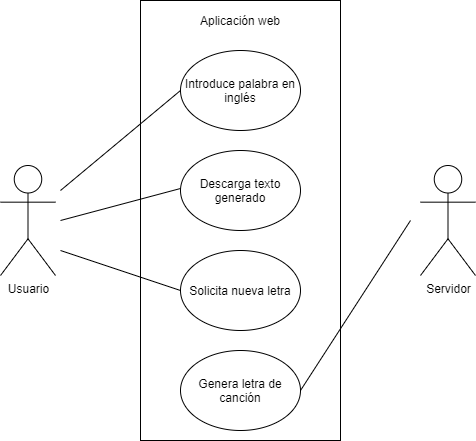
\includegraphics[width=13.5cm]{./Imagenes/Diagramas/CasoUso.png}
		\centering \caption{Diagrama de casos de uso}
	\end{figure}
	\newpage
	\begin{table}[hbt!]\caption{Caso de uso 1}% title of Table
		\centering % used for centering table
		\resizebox{13.5cm}{!} {
			\begin{tabular}{|c|c|}% centered columns (3 columns)
				\hline                        %inserts double horizontal lines
				\begin{tabular}[c]{@{}l@{}}Caso de uso\end{tabular}
				& \begin{tabular}[c]{@{}l@{}}Introduce palabra en inglés\end{tabular} \\% inserting body of the table 
				\hline				                     
				\begin{tabular}[c]{@{}l@{}}Actores\end{tabular}
				& \begin{tabular}[c]{@{}l@{}}Usuario\end{tabular} \\% inserting body of the table 
				\hline
				\begin{tabular}[c]{@{}l@{}}Descripción\end{tabular}
				& \begin{tabular}[c]{@{}l@{}}El usuario dentro de la aplicación web proporciona una palabra\\ en el idioma inglés para con ella poder generar un texto \end{tabular} \\
				\hline
			\end{tabular}\label{table:Caso de uso 1}% is used to refer this table in the text
		}
	\end{table}
	\begin{table}[hbt!]\caption{Caso de uso 2}% title of Table
		\centering % used for centering table
		\resizebox{13.5cm}{!} {
			\begin{tabular}{|c|c|}% centered columns (3 columns)
				\hline                        %inserts double horizontal lines
				\begin{tabular}[c]{@{}l@{}}Caso de uso\end{tabular}
				& \begin{tabular}[c]{@{}l@{}}Descargar texto generado\end{tabular} \\% inserting body of the table 
				\hline				                     
				\begin{tabular}[c]{@{}l@{}}Actores\end{tabular}
				& \begin{tabular}[c]{@{}l@{}}Usuario\end{tabular} \\% inserting body of the table 
				\hline
				\begin{tabular}[c]{@{}l@{}}Descripción\end{tabular}
				& \begin{tabular}[c]{@{}l@{}}El usuario dentro de la aplicación web tiene la posibilidad\\ de descargar el texto generado por el modelo  \end{tabular} \\
				\hline
			\end{tabular}\label{table:Caso de uso 2}% is used to refer this table in the text
		}
	\end{table}	
	\begin{table}[hbt!]\caption{Caso de uso 3}% title of Table
		\centering % used for centering table
		\resizebox{13.5cm}{!} {
			\begin{tabular}{|c|c|}% centered columns (3 columns)
				\hline                        %inserts double horizontal lines
				\begin{tabular}[c]{@{}l@{}}Caso de uso\end{tabular}
				& \begin{tabular}[c]{@{}l@{}}Solicitar nueva letra\end{tabular} \\% inserting body of the table 
				\hline				                     
				\begin{tabular}[c]{@{}l@{}}Actores\end{tabular}
				& \begin{tabular}[c]{@{}l@{}}Usuario\end{tabular} \\% inserting body of the table 
				\hline
				\begin{tabular}[c]{@{}l@{}}Descripción\end{tabular}
				& \begin{tabular}[c]{@{}l@{}}Al usuario dentro de la aplicación web se le da posibilidad de volver\\ a generar otra letra musical usando los mismos parámetros que proporcionó\\ o utilizando unos nuevos\end{tabular} \\
				\hline
			\end{tabular}\label{table:Caso de uso 3}% is used to refer this table in the text
		}
	\end{table}	
	\begin{table}[hbt!]\caption{Caso de uso 4}% title of Table
		\centering % used for centering table
		\resizebox{13.5cm}{!} {
			\begin{tabular}{|c|c|}% centered columns (3 columns)
				\hline                        %inserts double horizontal lines
				\begin{tabular}[c]{@{}l@{}}Caso de uso\end{tabular}
				& \begin{tabular}[c]{@{}l@{}}Genera letra de canción\end{tabular} \\% inserting body of the table 
				\hline				                     
				\begin{tabular}[c]{@{}l@{}}Actores\end{tabular}
				& \begin{tabular}[c]{@{}l@{}}Servidor\end{tabular} \\% inserting body of the table 
				\hline
				\begin{tabular}[c]{@{}l@{}}Descripción\end{tabular}
				& \begin{tabular}[c]{@{}l@{}}El servidor envia el texto generado por el modelo a la aplicación web,\\ la cual se encarga de mostrarla al usuario final \end{tabular} \\
				\hline
			\end{tabular}\label{table:Caso de uso41}% is used to refer this table in the text
		}
	\end{table}
	\newpage
	\section{Funcionamiento general del sistema}
	El siguiente diagrama muestra el funcionamiento general del producto, donde se ejemplifica a grandes rasgos la extracción del dataset con el cual, después de limpiarlo se realiza el entrenamiento del modelo, el cual puede generar textos, dichos textos en comunicación con el servidor web se muestran al usuario final.
	\begin{figure}[H] 
		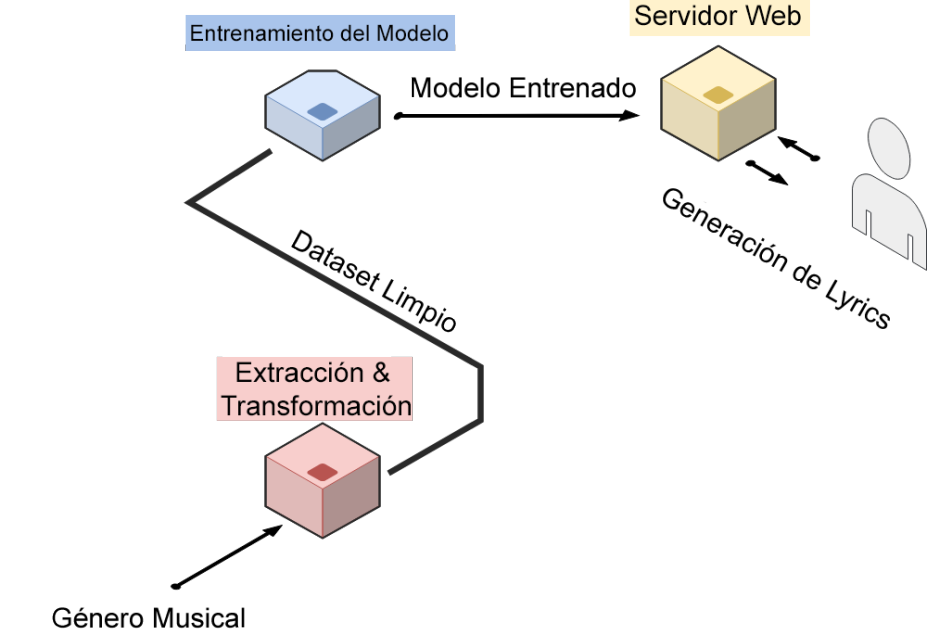
\includegraphics[width=13.5cm]{./Imagenes/Diagramas/general.png}
		\centering \caption{Diagrama general del sistema}
	\end{figure}
	\newpage
	\section{Aspecto técnico del desarrollo del sistema}
	\newpage
	\section{Desarrollo de la aplicación web}
	\newpage
	\section{Generación del modelo}
	\newpage
	\section{Conexión entre el modelo y la aplicación web}
	\newpage
	\begin{thebibliography}{20}
		\bibitem{refQuesPython} 
		Python (2021), What is Python? Executive Summary, [En línea]. Disponible: https://www.python.org/doc/essays/blurb/ [Último acceso: 24 de abril del 2021].
		\bibitem{refHtml}
		Mozilla.org (2021, febrero 19), HTML basics, [En línea]. Disponible: https://developer.mozilla.org/en-US/docs/Learn/Getting\_started\_with\_the\_web/HTML\_basics [Último acceso: 15 de mayo del 2021].
		\bibitem{refHtml2}
		Mozilla.org (2021, mayo 14), HTML5, [En línea]. Disponible: https://developer.mozilla.org/es/docs/Web/Guide/HTML/HTML5 [Último acceso: 15 de mayo del 2021].
		\bibitem{refcss}
		W3C (2016), HTML \& CSS, [En línea]. Disponible: [Último acceso: 15 de mayo del 2021].		
		\bibitem{refjs}
		Mozilla.org (2021, abril 27), What is JavaScript?, [En línea]. Disponible: https://developer.mozilla.org/en-US/docs/Learn/JavaScript/First\_steps/What\_is\_JavaScript [Último acceso: 15 de mayo del 2021].
		\bibitem{amazon_ec2}
		Amazon (2021), Amazon EC2 [En línea]. Disponible: https://aws.amazon.com/es/ec2/?ec2-whats-new.sort-by=item.additionalFields.postDateTime\&ec2-whats-new.sort-order=desc [Último acceso: 1 Junio 2021]		
		\bibitem{amazon_sagemaker}
		Amazon (2021), Amazon SageMaker [En línea]. Disponible: https://aws.amazon.com/es/sagemaker/ [Último acceso: 1 Junio 2021]		
		\bibitem{amazon_s3}
		Amazon (2021), Amazon S3 [En línea]. Disponible: https://aws.amazon.com/es/s3/ [Último acceso: 1 Junio 2021]
	\end{thebibliography}	
\end{document}